\section{Assignment 9}

\subsection{Design the operational space PD control law with gravity compensation}

\begin{figure}[H]
\centering
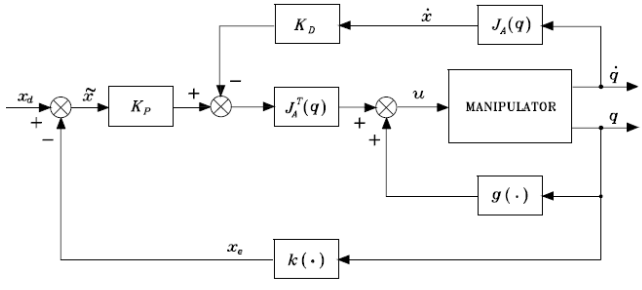
\includegraphics[keepaspectratio,width=0.4\textwidth]{op_pd_arch}
\caption{Operational space PD control law with gravity compensation architecture}
\end{figure}

The operational space PD control law with gravity compensation works exactly the same as the joint space one, except for the transformation of the joint space quantities into the corresponding operational space ones with direct kinematics (i.e. with the use of the transformation matrix $T$ and of the analytical Jacobian $JA$). The control law parameters are $K_P=50,K_D=10$. The architecture was tested with a constant pose reference obtained by applying direct kinematics to the joint configuration $q=\begin{bmatrix}
-\pi/3&-0.1&\pi/2
\end{bmatrix}$.

\begin{figure}[H]
\centering
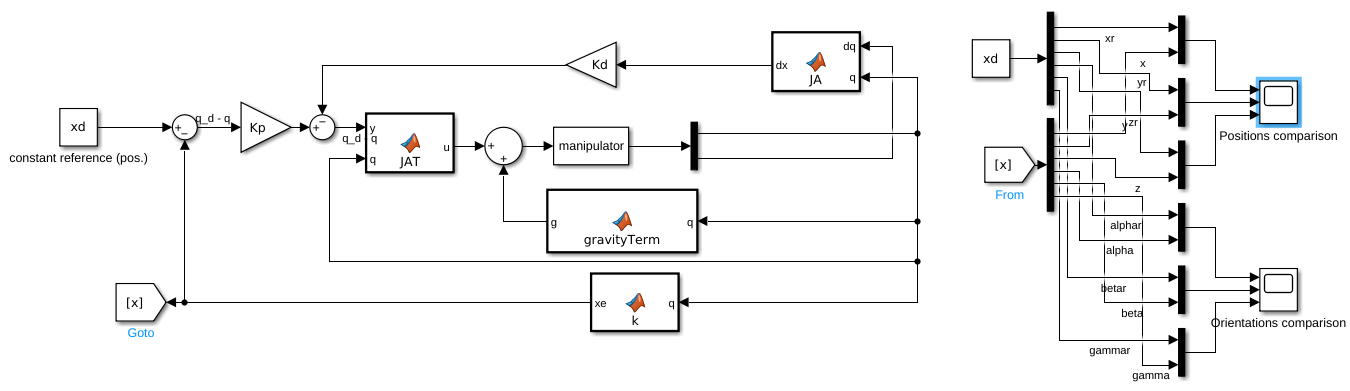
\includegraphics[keepaspectratio,width=0.7\textwidth]{op_pd_sim}
\caption{Operational space PD control law with gravity compensation SIMULINK model}
\end{figure}

\begin{figure}[H]
\begin{minipage}{0.5\textwidth}
\centering
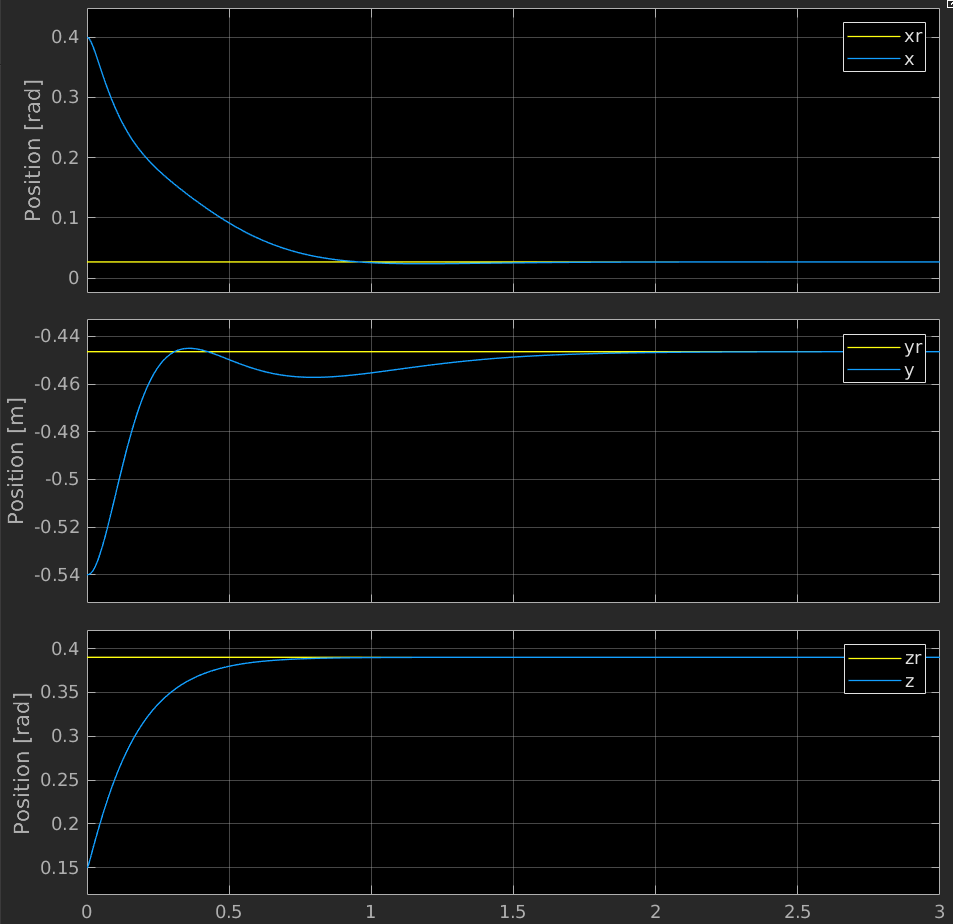
\includegraphics[keepaspectratio,width=\textwidth]{op_pd_pos}
\caption{Pose tracking - end-effector xyz coordinates}
\end{minipage}
\begin{minipage}{0.5\textwidth}
\centering
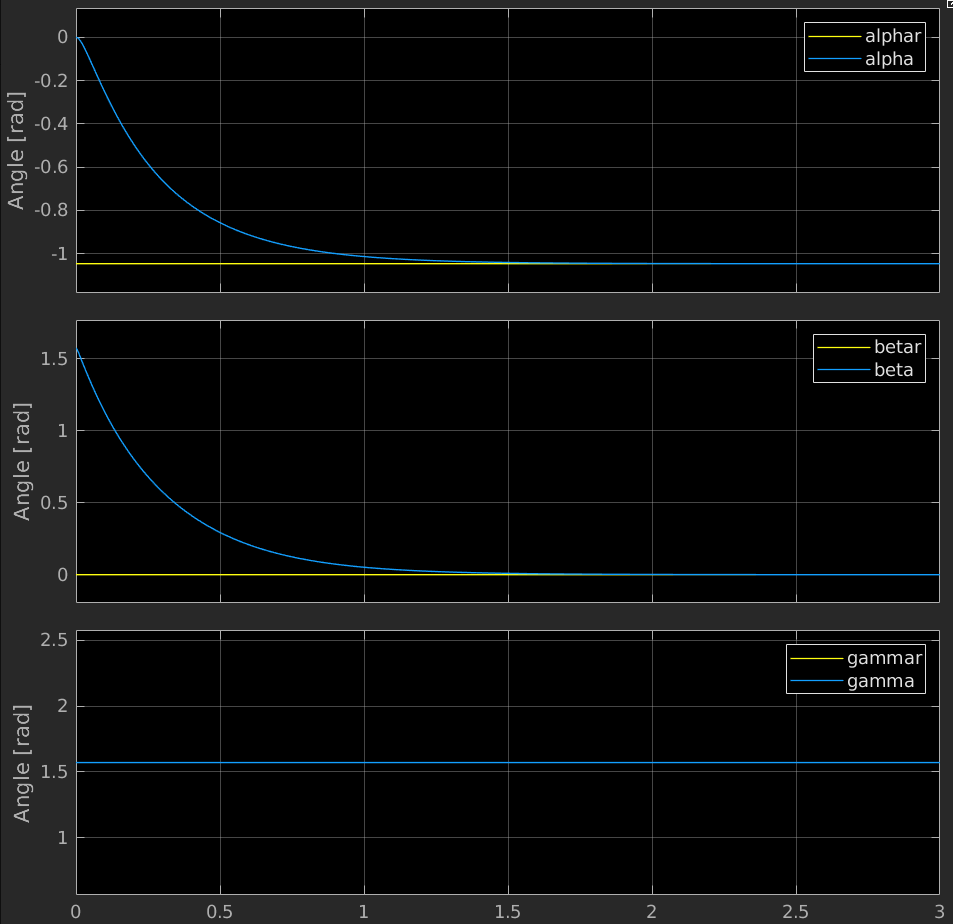
\includegraphics[keepaspectratio,width=\textwidth]{op_pd_or}
\caption{Pose tracking - end-effector $\alpha\beta\gamma$ coordinates}
\end{minipage}
\end{figure}